\documentclass[DM,lsstdraft,toc]{lsstdoc}
% lsstdoc documentation: https://lsst-texmf.lsst.io/lsstdoc.html

% Generated by Makefile
\input{meta}

% Package imports go here.
\usepackage{booktabs}
\usepackage{graphicx}

% Local commands go here.
\newcolumntype{R}[1]{>{\raggedleft\arraybackslash}p{#1}}
\newcolumntype{L}[1]{>{\raggedright\arraybackslash}p{#1}}

% If you want glossaries, uncomment:
% \input{aglossary.tex}
% \makeglossaries

\title{Characterization Metric Report: Science Pipelines Version 20.0.0}
% \setDocSubtitle{Optional subtitle}

\author{%
Jeff Carlin
}

\setDocRef{DMTR-251}
\setDocUpstreamLocation{\url{https://github.com/lsst-dm/DMTR-251}}
\date{\vcsDate}
% \setDocCurator{The Curator of this Document}

\setDocAbstract{%
This brief report describes measurements of interest that were carried out for release v20.0.0 of the Science Pipeline.
The report for the previous version can be found in \citeds{DMTR-191}.
}

% Revision history.
% Order: oldest first.
% Fields: VERSION, DATE, DESCRIPTION, OWNER NAME.
% See LPM-51 for version number policy.
\setDocChangeRecord{%
  \addtohist{1}{2020-06-16}{First Draft}{Jeff Carlin}
}

\begin{document}

\maketitle

% ADD CONTENT HERE
% You can also use the \input command to include several content files.

The Characterization Metric Report that has accompanied previous releases of the Science Pipelines (through v19.0) has typically contained metrics that were measured using \href{https://github.com/lsst/validation_data_hsc}{validation\_data\_hsc}. This test dataset consists of 8 HSC engineering images: 2 \emph{r}-band, 4 \emph{i}'-band, and 2 \emph{y}-band. For continuity with previous releases, we report metrics from validation\_data\_hsc in this document, but we will use a more substantial dataset for characterization of future releases. For this small dataset, metric measurements were made on individual, separately-processed, single-frame images: jointcal was not run. All values were computed using the \texttt{examples/runHscTest.sh} script in the \href{https://github.com/lsst/validate_drp}{validate\_drp} package.

In this report, we also show metrics measured on the HSC-RC2 dataset. RC2 consists of 3 tracts of data taken from the HSC-SSP survey, and selected to provide a means of testing various ``pathological'' cases (e.g., difficult astrometric solutions, seeing too small to provide a well-sampled PSF, difficult fields for deblending, and large galaxies, among others). These three tracts each contain between 112--149 visits split between the HSC-G, HSC-R, HSC-I, HSC-Z, and HSC-Y (\emph{grizy}) filters. The validate\_drp scripts were run on these tracts to derive a total of 14 photometric, astrometric, and shape metrics, a subset of which are reported here. We exclude the three astrometry metrics (AM3, AD3, and AF3) that concern residuals on 200-arcminute scales, since neither the handful of CCDs in the validation\_data\_hsc dataset nor the individual tracts of RC2 span large enough spatial scales to enable these measurements. The RC2 data processing includes jointcal, and thus provides a better representation of the state of the science pipelines than the much simpler validation\_data\_hsc runs.

For comparison, we provide the \SRD required ``design'' value of each metric as defined in the Science Requirements Document \citedsp{LPM-17}, and, where available, the target for this release as defined in the Data Management Development Milestone Roadmap \citedsp{LDM-240}. For context, the \SRD does not place any constraints on \emph{y}-band for these KPMs.  For the photometric metrics, there are only specifications for \emph{g}, \emph{r}, and \emph{i}'. In the case of the ellipticity correlation metrics, there are specs only for \emph{r} and \emph{i}'. The \emph{y}-band measurements are for interest and historical tracking.

Some KPMs (AF1, AD1) involve thresholds that are different for ``design'', ``minimum'', and ``stretch'' specifications. The metrics in this report are all compared to the ``design'' thresholds. The assessment of these KPMs would be different if evaluated against different thresholds.

The per-cycle target numbers come from the ``KPMs'' sheet of \href{http://ls.st/LDM-240}{LDM-240}.

\section{Dashboard summary of performance metrics}

Metrics are typically monitored on a dashboard hosted by SQuaSH (Science Quality System Harness; described in \citedsp{sqr-009}). Here we show an example of this dashboard displaying $\sim4$ months of measurements for a few metrics. These measurements are for tract 9813, as measured in the \emph{r}-band filter (HSC-R). Note that the large increase between April-June was due to some bugs and issues in the codebase that have since been identified and fixed. The metric values in the most recent processing (with the v20.0 release candidate dubbed v20\_0\_0\_rc1) have returned to similar levels to early 2020.

\begin{figure}
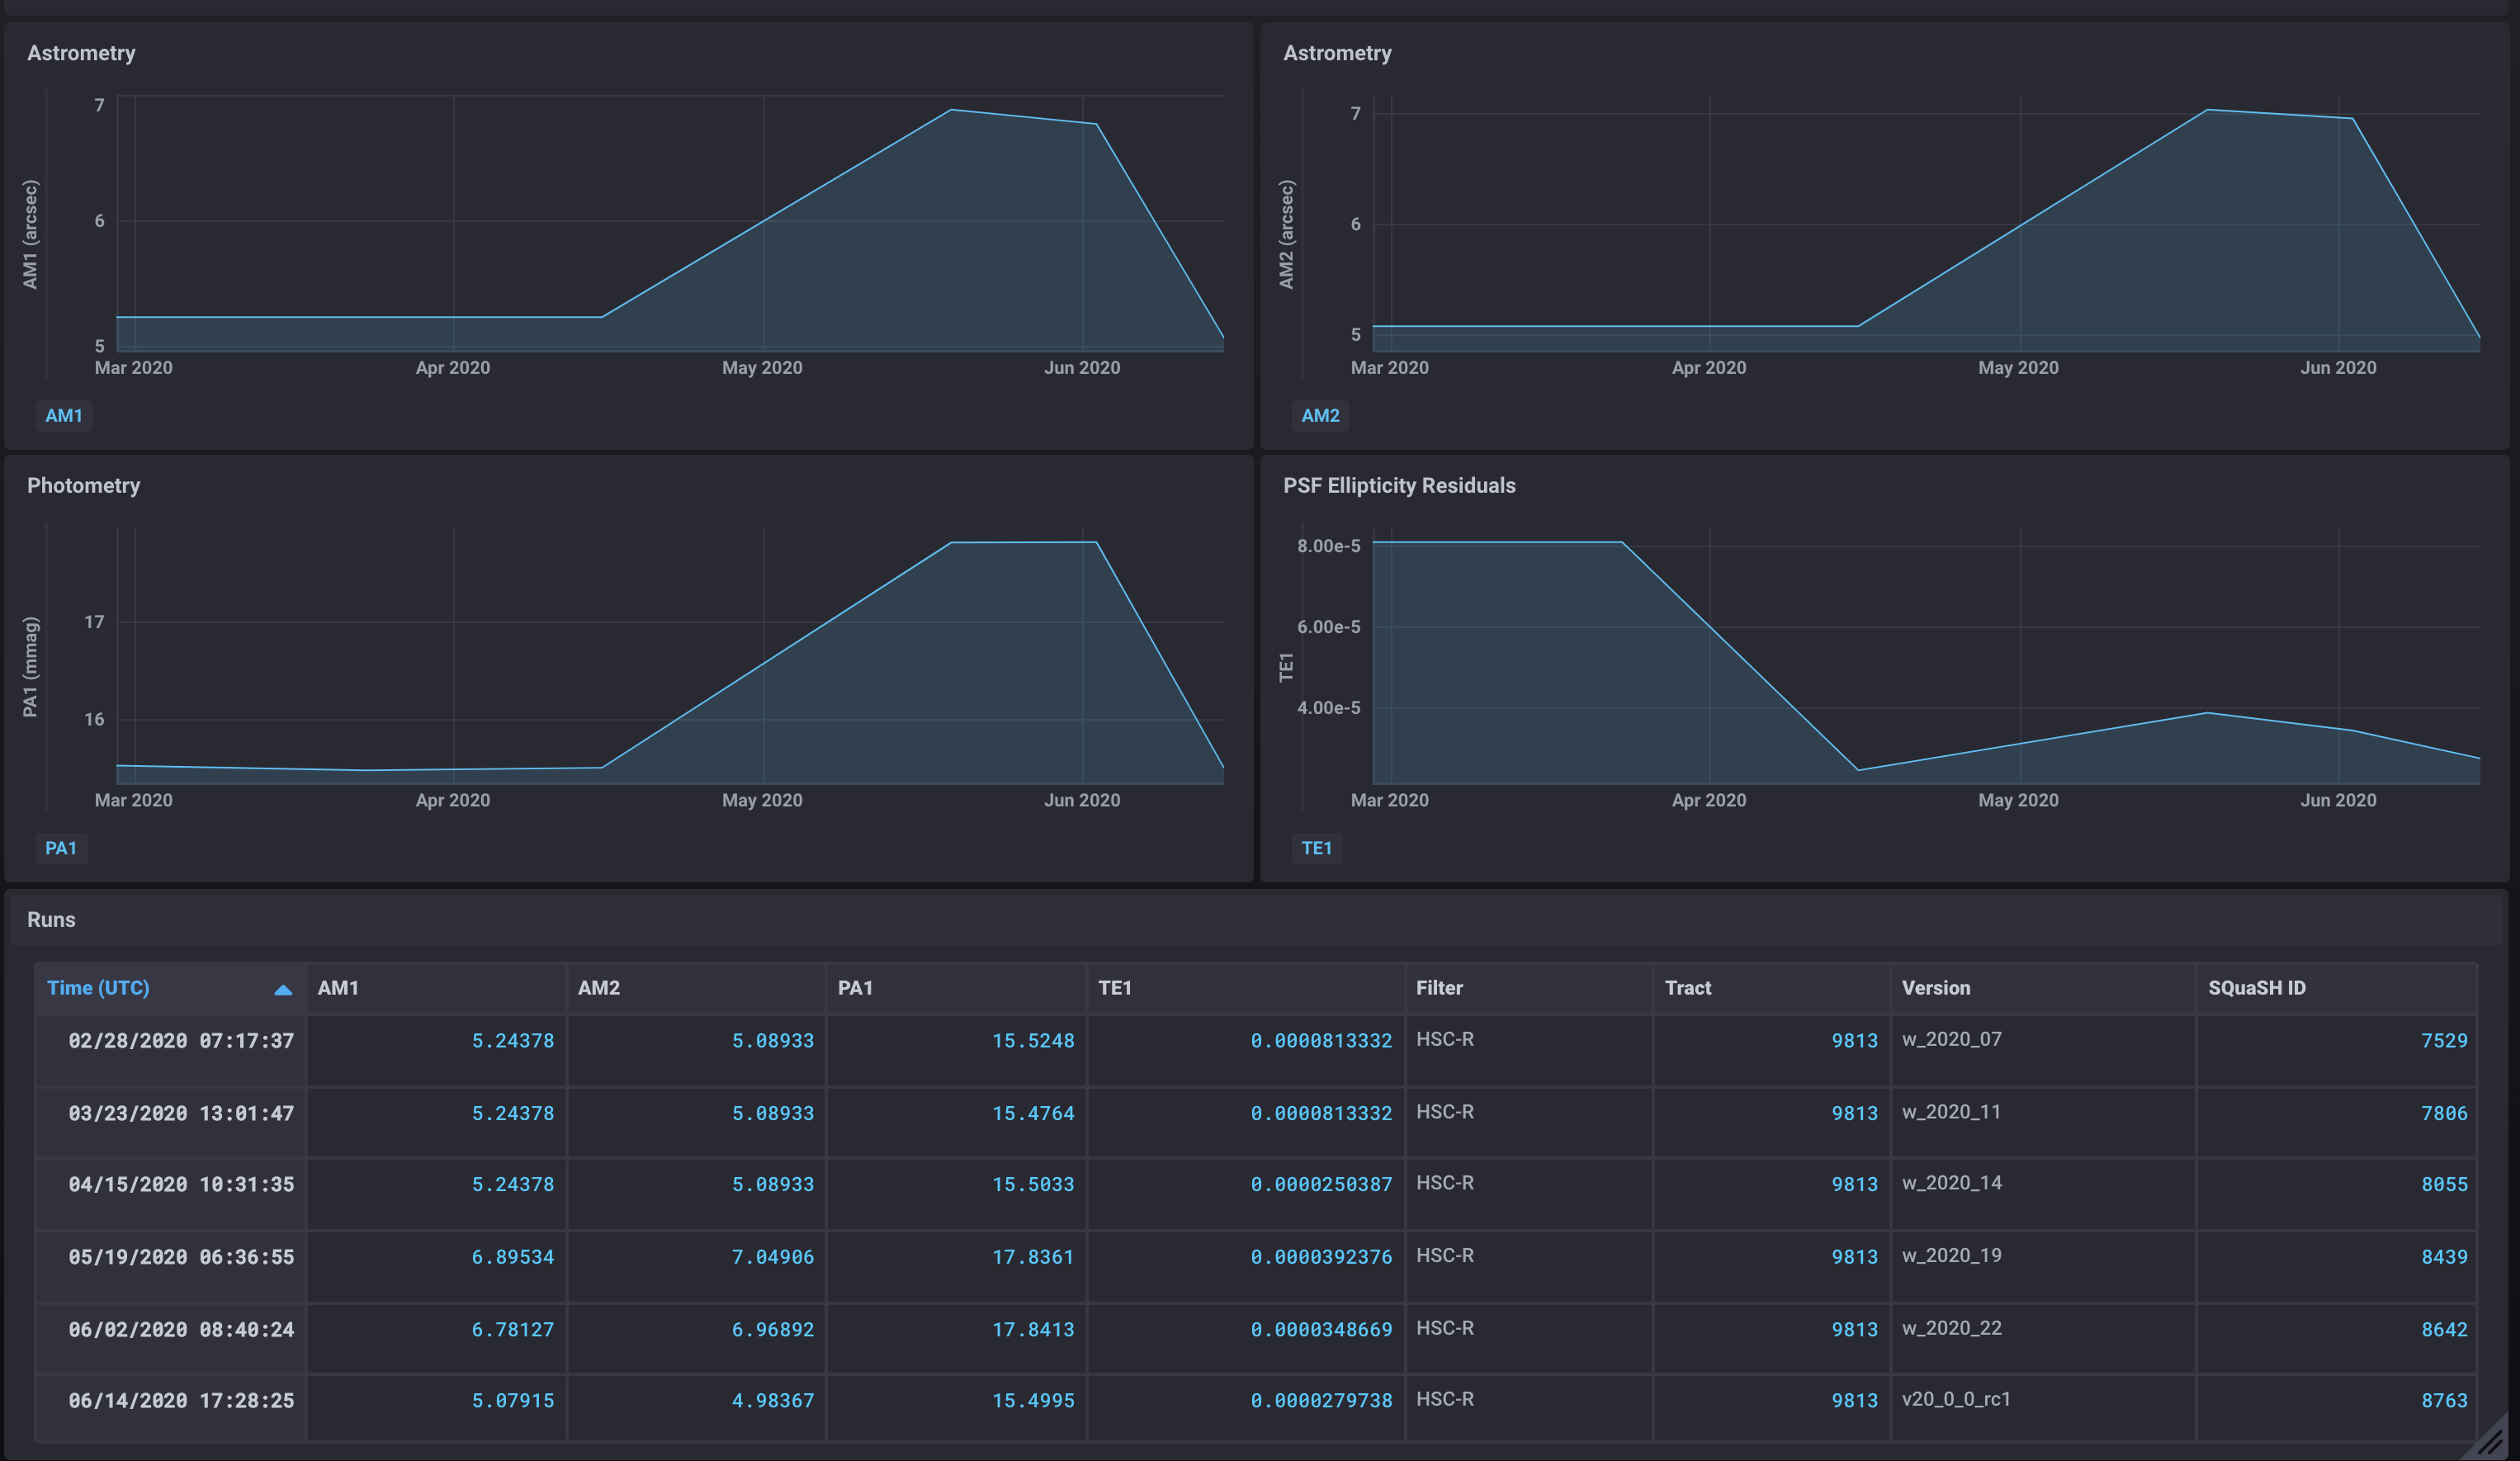
\includegraphics[width=1.0\columnwidth]{figures/SQuaSH_dashboard_RC2_tract9813.png}
\caption{SQuaSH dashboard showing the past four months of metric measurements from the RC2 dataset. This view shows the metrics for tract 9813 in the HSC-R filter. The ``regression'' in the metrics from April-June was due to some bugs and configuration changes. After all of these were repaired, the metric values as calculated by the v20.0 science pipelines returned to the levels they were at before those bugs.}
\end{figure}

\section{Photometric Performance}\label{photometric-performance}

procCalRep corresponds to requirement OSS-REQ-0275 (defined in
\citeds{LSE-30}). All other photometric performance
metrics follow LSS-REQ-0093 (\citeds{LSE-29}) and Table 14 of \citeds{LPM-17}.

Any entries left blank are those for which we do not have data in the given filter for that dataset.

\begin{longtable}[]{@{}lllllll@{}}
\toprule
\begin{minipage}[b]{0.12\columnwidth}\raggedright\strut
Metric\strut
\end{minipage} & \begin{minipage}[b]{0.06\columnwidth}\raggedright\strut
Unit\strut
\end{minipage} & \begin{minipage}[b]{0.14\columnwidth}\raggedright\strut
SRD Requirement -- Design\strut
\end{minipage} & \begin{minipage}[b]{0.14\columnwidth}\raggedright\strut
Release 20 Target\strut
\end{minipage} & \begin{minipage}[b]{0.12\columnwidth}\raggedright\strut
Value (validation data)\strut
\end{minipage} & \begin{minipage}[b]{0.12\columnwidth}\raggedright\strut
Value (RC2) \strut
\end{minipage} & \begin{minipage}[b]{0.17\columnwidth}\raggedright\strut
Comments\strut
\end{minipage}\tabularnewline
\midrule
\endhead
\begin{minipage}[t]{0.12\columnwidth}\raggedright\strut
procCalRep\strut
\end{minipage} & \begin{minipage}[t]{0.06\columnwidth}\raggedright\strut
mmag\strut
\end{minipage} & \begin{minipage}[t]{0.14\columnwidth}\raggedright\strut
\(\leq 3.0\)\strut
\end{minipage} & \begin{minipage}[t]{0.14\columnwidth}\raggedright\strut
3.5\strut
\end{minipage} & \begin{minipage}[t]{0.12\columnwidth}\raggedright\strut
---\strut
\end{minipage} & \begin{minipage}[t]{0.12\columnwidth}\raggedright\strut
---\strut
\end{minipage} & \begin{minipage}[t]{0.17\columnwidth}\raggedright\strut
Need simulations\strut
\end{minipage}\tabularnewline
\begin{minipage}[t]{0.12\columnwidth}\raggedright\strut
PA1: \emph{u}\strut
\end{minipage} & \begin{minipage}[t]{0.06\columnwidth}\raggedright\strut
mmag\strut
\end{minipage} & \begin{minipage}[t]{0.14\columnwidth}\raggedright\strut
\(\leq 7.5\)\strut
\end{minipage} & \begin{minipage}[t]{0.14\columnwidth}\raggedright\strut
8.0\strut
\end{minipage} & \begin{minipage}[t]{0.12\columnwidth}\raggedright\strut
---\strut
\end{minipage} & \begin{minipage}[t]{0.12\columnwidth}\raggedright\strut
--- \strut
\end{minipage} & \begin{minipage}[t]{0.17\columnwidth}\raggedright\strut
No data\strut
\end{minipage}\tabularnewline
\begin{minipage}[t]{0.12\columnwidth}\raggedright\strut
PA1: \emph{g}\strut
\end{minipage} & \begin{minipage}[t]{0.06\columnwidth}\raggedright\strut
mmag\strut
\end{minipage} & \begin{minipage}[t]{0.14\columnwidth}\raggedright\strut
\(\leq 5.0\)\strut
\end{minipage} & \begin{minipage}[t]{0.14\columnwidth}\raggedright\strut
5.5\strut
\end{minipage} & \begin{minipage}[t]{0.12\columnwidth}\raggedright\strut
---\strut
\end{minipage} & \begin{minipage}[t]{0.12\columnwidth}\raggedright\strut
12.7 \strut
\end{minipage} & \begin{minipage}[t]{0.17\columnwidth}\raggedright\strut
\strut
\end{minipage}\tabularnewline
\begin{minipage}[t]{0.12\columnwidth}\raggedright\strut
PA1: \emph{r}\strut
\end{minipage} & \begin{minipage}[t]{0.06\columnwidth}\raggedright\strut
mmag\strut
\end{minipage} & \begin{minipage}[t]{0.14\columnwidth}\raggedright\strut
\(\leq 5.0\)\strut
\end{minipage} & \begin{minipage}[t]{0.14\columnwidth}\raggedright\strut
5.5\strut
\end{minipage} & \begin{minipage}[t]{0.12\columnwidth}\raggedright\strut
13.7\strut
\end{minipage} & \begin{minipage}[t]{0.12\columnwidth}\raggedright\strut
14.1\strut
\end{minipage} & \begin{minipage}[t]{0.17\columnwidth}\raggedright\strut
\strut
\end{minipage}\tabularnewline
\begin{minipage}[t]{0.12\columnwidth}\raggedright\strut
PA1: \emph{i}\strut
\end{minipage} & \begin{minipage}[t]{0.06\columnwidth}\raggedright\strut
mmag\strut
\end{minipage} & \begin{minipage}[t]{0.14\columnwidth}\raggedright\strut
\(\leq 5.0\)\strut
\end{minipage} & \begin{minipage}[t]{0.14\columnwidth}\raggedright\strut
5.5\strut
\end{minipage} & \begin{minipage}[t]{0.12\columnwidth}\raggedright\strut
12.1\strut
\end{minipage} & \begin{minipage}[t]{0.12\columnwidth}\raggedright\strut
14.0\strut
\end{minipage} & \begin{minipage}[t]{0.17\columnwidth}\raggedright\strut
\strut
\end{minipage}\tabularnewline
\begin{minipage}[t]{0.12\columnwidth}\raggedright\strut
PA1: \emph{z}\strut
\end{minipage} & \begin{minipage}[t]{0.06\columnwidth}\raggedright\strut
mmag\strut
\end{minipage} & \begin{minipage}[t]{0.14\columnwidth}\raggedright\strut
\(\leq 7.5\)\strut
\end{minipage} & \begin{minipage}[t]{0.14\columnwidth}\raggedright\strut
8.0\strut
\end{minipage} & \begin{minipage}[t]{0.12\columnwidth}\raggedright\strut
---\strut
\end{minipage} & \begin{minipage}[t]{0.12\columnwidth}\raggedright\strut
11.6\strut
\end{minipage} & \begin{minipage}[t]{0.17\columnwidth}\raggedright\strut
\strut
\end{minipage}\tabularnewline
\begin{minipage}[t]{0.12\columnwidth}\raggedright\strut
PA1: \emph{y}\strut
\end{minipage} & \begin{minipage}[t]{0.06\columnwidth}\raggedright\strut
mmag\strut
\end{minipage} & \begin{minipage}[t]{0.14\columnwidth}\raggedright\strut
\(\leq 7.5\)\strut
\end{minipage} & \begin{minipage}[t]{0.14\columnwidth}\raggedright\strut
8.0\strut
\end{minipage} & \begin{minipage}[t]{0.12\columnwidth}\raggedright\strut
23.8\strut
\end{minipage} & \begin{minipage}[t]{0.12\columnwidth}\raggedright\strut
13.5\strut
\end{minipage} & \begin{minipage}[t]{0.17\columnwidth}\raggedright\strut
\strut
\end{minipage}\tabularnewline
\begin{minipage}[t]{0.12\columnwidth}\raggedright\strut
PF1: \emph{u}\strut
\end{minipage} & \begin{minipage}[t]{0.06\columnwidth}\raggedright\strut
\%\strut
\end{minipage} & \begin{minipage}[t]{0.14\columnwidth}\raggedright\strut
\(\leq 20\)\strut
\end{minipage} & \begin{minipage}[t]{0.14\columnwidth}\raggedright\strut
20.0\strut
\end{minipage} & \begin{minipage}[t]{0.12\columnwidth}\raggedright\strut
---\strut
\end{minipage} & \begin{minipage}[t]{0.12\columnwidth}\raggedright\strut
---\strut
\end{minipage} & \begin{minipage}[t]{0.17\columnwidth}\raggedright\strut
No data\strut
\end{minipage}\tabularnewline
\begin{minipage}[t]{0.12\columnwidth}\raggedright\strut
PF1: \emph{g}\strut
\end{minipage} & \begin{minipage}[t]{0.06\columnwidth}\raggedright\strut
\%\strut
\end{minipage} & \begin{minipage}[t]{0.14\columnwidth}\raggedright\strut
\(\leq 20\)\strut
\end{minipage} & \begin{minipage}[t]{0.14\columnwidth}\raggedright\strut
20.0\strut
\end{minipage} & \begin{minipage}[t]{0.12\columnwidth}\raggedright\strut
---\strut
\end{minipage} & \begin{minipage}[t]{0.12\columnwidth}\raggedright\strut
28.6\strut
\end{minipage} & \begin{minipage}[t]{0.17\columnwidth}\raggedright\strut
\strut
\end{minipage}\tabularnewline
\begin{minipage}[t]{0.12\columnwidth}\raggedright\strut
PF1: \emph{r}\strut
\end{minipage} & \begin{minipage}[t]{0.06\columnwidth}\raggedright\strut
\%\strut
\end{minipage} & \begin{minipage}[t]{0.14\columnwidth}\raggedright\strut
\(\leq 10\)\strut
\end{minipage} & \begin{minipage}[t]{0.14\columnwidth}\raggedright\strut
10.0\strut
\end{minipage} & \begin{minipage}[t]{0.12\columnwidth}\raggedright\strut
30.1\strut
\end{minipage} & \begin{minipage}[t]{0.12\columnwidth}\raggedright\strut
31.1\strut
\end{minipage} & \begin{minipage}[t]{0.17\columnwidth}\raggedright\strut
\strut
\end{minipage}\tabularnewline
\begin{minipage}[t]{0.12\columnwidth}\raggedright\strut
PF1: \emph{i}\strut
\end{minipage} & \begin{minipage}[t]{0.06\columnwidth}\raggedright\strut
\%\strut
\end{minipage} & \begin{minipage}[t]{0.14\columnwidth}\raggedright\strut
\(\leq 10\)\strut
\end{minipage} & \begin{minipage}[t]{0.14\columnwidth}\raggedright\strut
10.0\strut
\end{minipage} & \begin{minipage}[t]{0.12\columnwidth}\raggedright\strut
25.9\strut
\end{minipage} & \begin{minipage}[t]{0.12\columnwidth}\raggedright\strut
31.7\strut
\end{minipage} & \begin{minipage}[t]{0.17\columnwidth}\raggedright\strut
\strut
\end{minipage}\tabularnewline
\begin{minipage}[t]{0.12\columnwidth}\raggedright\strut
PF1: \emph{z}\strut
\end{minipage} & \begin{minipage}[t]{0.06\columnwidth}\raggedright\strut
\%\strut
\end{minipage} & \begin{minipage}[t]{0.14\columnwidth}\raggedright\strut
\(\leq 20\)\strut
\end{minipage} & \begin{minipage}[t]{0.14\columnwidth}\raggedright\strut
20.0\strut
\end{minipage} & \begin{minipage}[t]{0.12\columnwidth}\raggedright\strut
---\strut
\end{minipage} & \begin{minipage}[t]{0.12\columnwidth}\raggedright\strut
13.2\strut
\end{minipage} & \begin{minipage}[t]{0.17\columnwidth}\raggedright\strut
\strut
\end{minipage}\tabularnewline
\begin{minipage}[t]{0.12\columnwidth}\raggedright\strut
PF1: \emph{y}\strut
\end{minipage} & \begin{minipage}[t]{0.06\columnwidth}\raggedright\strut
\%\strut
\end{minipage} & \begin{minipage}[t]{0.14\columnwidth}\raggedright\strut
\(\leq 10\)\strut
\end{minipage} & \begin{minipage}[t]{0.14\columnwidth}\raggedright\strut
10.0\strut
\end{minipage} & \begin{minipage}[t]{0.12\columnwidth}\raggedright\strut
34.7\strut
\end{minipage} & \begin{minipage}[t]{0.12\columnwidth}\raggedright\strut
16.6\strut
\end{minipage} & \begin{minipage}[t]{0.17\columnwidth}\raggedright\strut
\strut
\end{minipage}\tabularnewline
\begin{minipage}[t]{0.12\columnwidth}\raggedright\strut
PA2: \emph{u}\strut
\end{minipage} & \begin{minipage}[t]{0.06\columnwidth}\raggedright\strut
\%\strut
\end{minipage} & \begin{minipage}[t]{0.14\columnwidth}\raggedright\strut
\(\leq 22.5\)\strut
\end{minipage} & \begin{minipage}[t]{0.14\columnwidth}\raggedright\strut
---\strut
\end{minipage} & \begin{minipage}[t]{0.12\columnwidth}\raggedright\strut
---\strut
\end{minipage} & \begin{minipage}[t]{0.12\columnwidth}\raggedright\strut
---\strut
\end{minipage} & \begin{minipage}[t]{0.17\columnwidth}\raggedright\strut
No data\strut
\end{minipage}\tabularnewline
\begin{minipage}[t]{0.12\columnwidth}\raggedright\strut
PA2: \emph{g}\strut
\end{minipage} & \begin{minipage}[t]{0.06\columnwidth}\raggedright\strut
\%\strut
\end{minipage} & \begin{minipage}[t]{0.14\columnwidth}\raggedright\strut
\(\leq 15\)\strut
\end{minipage} & \begin{minipage}[t]{0.14\columnwidth}\raggedright\strut
---\strut
\end{minipage} & \begin{minipage}[t]{0.12\columnwidth}\raggedright\strut
---\strut
\end{minipage} & \begin{minipage}[t]{0.12\columnwidth}\raggedright\strut
27.9\strut
\end{minipage} & \begin{minipage}[t]{0.17\columnwidth}\raggedright\strut
\strut
\end{minipage}\tabularnewline
\begin{minipage}[t]{0.12\columnwidth}\raggedright\strut
PA2: \emph{r}\strut
\end{minipage} & \begin{minipage}[t]{0.06\columnwidth}\raggedright\strut
\%\strut
\end{minipage} & \begin{minipage}[t]{0.14\columnwidth}\raggedright\strut
\(\leq 15\)\strut
\end{minipage} & \begin{minipage}[t]{0.14\columnwidth}\raggedright\strut
20.0\strut
\end{minipage} & \begin{minipage}[t]{0.12\columnwidth}\raggedright\strut
26.6\strut
\end{minipage} & \begin{minipage}[t]{0.12\columnwidth}\raggedright\strut
29.8\strut
\end{minipage} & \begin{minipage}[t]{0.17\columnwidth}\raggedright\strut
\strut
\end{minipage}\tabularnewline
\begin{minipage}[t]{0.12\columnwidth}\raggedright\strut
PA2: \emph{i}\strut
\end{minipage} & \begin{minipage}[t]{0.06\columnwidth}\raggedright\strut
\%\strut
\end{minipage} & \begin{minipage}[t]{0.14\columnwidth}\raggedright\strut
\(\leq 15\)\strut
\end{minipage} & \begin{minipage}[t]{0.14\columnwidth}\raggedright\strut
20.0\strut
\end{minipage} & \begin{minipage}[t]{0.12\columnwidth}\raggedright\strut
25.4\strut
\end{minipage} & \begin{minipage}[t]{0.12\columnwidth}\raggedright\strut
29.7\strut
\end{minipage} & \begin{minipage}[t]{0.17\columnwidth}\raggedright\strut
\strut
\end{minipage}\tabularnewline
\begin{minipage}[t]{0.12\columnwidth}\raggedright\strut
PA2: \emph{z}\strut
\end{minipage} & \begin{minipage}[t]{0.06\columnwidth}\raggedright\strut
\%\strut
\end{minipage} & \begin{minipage}[t]{0.14\columnwidth}\raggedright\strut
\(\leq 22.5\)\strut
\end{minipage} & \begin{minipage}[t]{0.14\columnwidth}\raggedright\strut
---\strut
\end{minipage} & \begin{minipage}[t]{0.12\columnwidth}\raggedright\strut
---\strut
\end{minipage} & \begin{minipage}[t]{0.12\columnwidth}\raggedright\strut
25.5\strut
\end{minipage} & \begin{minipage}[t]{0.17\columnwidth}\raggedright\strut
\strut
\end{minipage}\tabularnewline
\begin{minipage}[t]{0.12\columnwidth}\raggedright\strut
PA2: \emph{y}\strut
\end{minipage} & \begin{minipage}[t]{0.06\columnwidth}\raggedright\strut
\%\strut
\end{minipage} & \begin{minipage}[t]{0.14\columnwidth}\raggedright\strut
\(\leq 22.5\)\strut
\end{minipage} & \begin{minipage}[t]{0.14\columnwidth}\raggedright\strut
22.5\strut
\end{minipage} & \begin{minipage}[t]{0.12\columnwidth}\raggedright\strut
41.3\strut
\end{minipage} & \begin{minipage}[t]{0.12\columnwidth}\raggedright\strut
29.6\strut
\end{minipage} & \begin{minipage}[t]{0.17\columnwidth}\raggedright\strut
\strut
\end{minipage}\tabularnewline
\bottomrule
\end{longtable}

\section{Astrometric Performance}\label{astrometric-performance}

The following metrics are defined following LSR-REQ-0094
\citedsp{LSE-29} and Table 18 of \citeds{LPM-17}.

\begin{longtable}[]{@{}lllllll@{}}
\toprule
\begin{minipage}[b]{0.12\columnwidth}\raggedright\strut
Metric\strut
\end{minipage} & \begin{minipage}[b]{0.06\columnwidth}\raggedright\strut
Unit\strut
\end{minipage} & \begin{minipage}[b]{0.14\columnwidth}\raggedright\strut
SRD Requirement -- Design\strut
\end{minipage} & \begin{minipage}[b]{0.14\columnwidth}\raggedright\strut
Release 20 Target\strut
\end{minipage} & \begin{minipage}[b]{0.12\columnwidth}\raggedright\strut
Value (validation data)\strut
\end{minipage} & \begin{minipage}[b]{0.12\columnwidth}\raggedright\strut
Value (RC2) \strut
\end{minipage} & \begin{minipage}[b]{0.17\columnwidth}\raggedright\strut
Comments\strut
\end{minipage}\tabularnewline
\midrule
\endhead
\begin{minipage}[t]{0.12\columnwidth}\raggedright\strut
AM1: \emph{u}\strut
\end{minipage} & \begin{minipage}[t]{0.06\columnwidth}\raggedright\strut
mas\strut
\end{minipage} & \begin{minipage}[t]{0.14\columnwidth}\raggedright\strut
\(\leq 10\)\strut
\end{minipage} & \begin{minipage}[t]{0.14\columnwidth}\raggedright\strut
15.0\strut
\end{minipage} & \begin{minipage}[t]{0.12\columnwidth}\raggedright\strut
---\strut
\end{minipage} & \begin{minipage}[t]{0.12\columnwidth}\raggedright\strut
--- \strut
\end{minipage} & \begin{minipage}[t]{0.17\columnwidth}\raggedright\strut
No data\strut
\end{minipage}\tabularnewline
\begin{minipage}[t]{0.12\columnwidth}\raggedright\strut
AM1: \emph{g}\strut
\end{minipage} & \begin{minipage}[t]{0.06\columnwidth}\raggedright\strut
mas\strut
\end{minipage} & \begin{minipage}[t]{0.14\columnwidth}\raggedright\strut
\(\leq 10\)\strut
\end{minipage} & \begin{minipage}[t]{0.14\columnwidth}\raggedright\strut
15.0\strut
\end{minipage} & \begin{minipage}[t]{0.12\columnwidth}\raggedright\strut
---\strut
\end{minipage} & \begin{minipage}[t]{0.12\columnwidth}\raggedright\strut
4.9 \strut
\end{minipage} & \begin{minipage}[t]{0.17\columnwidth}\raggedright\strut
\strut
\end{minipage}\tabularnewline
\begin{minipage}[t]{0.12\columnwidth}\raggedright\strut
AM1: \emph{r}\strut
\end{minipage} & \begin{minipage}[t]{0.06\columnwidth}\raggedright\strut
mas\strut
\end{minipage} & \begin{minipage}[t]{0.14\columnwidth}\raggedright\strut
\(\leq 10\)\strut
\end{minipage} & \begin{minipage}[t]{0.14\columnwidth}\raggedright\strut
15.0\strut
\end{minipage} & \begin{minipage}[t]{0.12\columnwidth}\raggedright\strut
5.2\strut
\end{minipage} & \begin{minipage}[t]{0.12\columnwidth}\raggedright\strut
5.2\strut
\end{minipage} & \begin{minipage}[t]{0.17\columnwidth}\raggedright\strut
\strut
\end{minipage}\tabularnewline
\begin{minipage}[t]{0.12\columnwidth}\raggedright\strut
AM1: \emph{i}\strut
\end{minipage} & \begin{minipage}[t]{0.06\columnwidth}\raggedright\strut
mas\strut
\end{minipage} & \begin{minipage}[t]{0.14\columnwidth}\raggedright\strut
\(\leq 10\)\strut
\end{minipage} & \begin{minipage}[t]{0.14\columnwidth}\raggedright\strut
15.0\strut
\end{minipage} & \begin{minipage}[t]{0.12\columnwidth}\raggedright\strut
9.3\strut
\end{minipage} & \begin{minipage}[t]{0.12\columnwidth}\raggedright\strut
4.5\strut
\end{minipage} & \begin{minipage}[t]{0.17\columnwidth}\raggedright\strut
\strut
\end{minipage}\tabularnewline
\begin{minipage}[t]{0.12\columnwidth}\raggedright\strut
AM1: \emph{z}\strut
\end{minipage} & \begin{minipage}[t]{0.06\columnwidth}\raggedright\strut
mas\strut
\end{minipage} & \begin{minipage}[t]{0.14\columnwidth}\raggedright\strut
\(\leq 10\)\strut
\end{minipage} & \begin{minipage}[t]{0.14\columnwidth}\raggedright\strut
15.0\strut
\end{minipage} & \begin{minipage}[t]{0.12\columnwidth}\raggedright\strut
---\strut
\end{minipage} & \begin{minipage}[t]{0.12\columnwidth}\raggedright\strut
4.8\strut
\end{minipage} & \begin{minipage}[t]{0.17\columnwidth}\raggedright\strut
\strut
\end{minipage}\tabularnewline
\begin{minipage}[t]{0.12\columnwidth}\raggedright\strut
AM1: \emph{y}\strut
\end{minipage} & \begin{minipage}[t]{0.06\columnwidth}\raggedright\strut
mas\strut
\end{minipage} & \begin{minipage}[t]{0.14\columnwidth}\raggedright\strut
\(\leq 10\)\strut
\end{minipage} & \begin{minipage}[t]{0.14\columnwidth}\raggedright\strut
15.0\strut
\end{minipage} & \begin{minipage}[t]{0.12\columnwidth}\raggedright\strut
8.5\strut
\end{minipage} & \begin{minipage}[t]{0.12\columnwidth}\raggedright\strut
6.7\strut
\end{minipage} & \begin{minipage}[t]{0.17\columnwidth}\raggedright\strut
\strut
\end{minipage}\tabularnewline
\begin{minipage}[t]{0.12\columnwidth}\raggedright\strut
AF1: \emph{u}\strut
\end{minipage} & \begin{minipage}[t]{0.06\columnwidth}\raggedright\strut
\%\strut
\end{minipage} & \begin{minipage}[t]{0.14\columnwidth}\raggedright\strut
\(\leq 10\)\strut
\end{minipage} & \begin{minipage}[t]{0.14\columnwidth}\raggedright\strut
10.0\strut
\end{minipage} & \begin{minipage}[t]{0.12\columnwidth}\raggedright\strut
---\strut
\end{minipage} & \begin{minipage}[t]{0.12\columnwidth}\raggedright\strut
---\strut
\end{minipage} & \begin{minipage}[t]{0.17\columnwidth}\raggedright\strut
No data\strut
\end{minipage}\tabularnewline
\begin{minipage}[t]{0.12\columnwidth}\raggedright\strut
AF1: \emph{g}\strut
\end{minipage} & \begin{minipage}[t]{0.06\columnwidth}\raggedright\strut
\%\strut
\end{minipage} & \begin{minipage}[t]{0.14\columnwidth}\raggedright\strut
\(\leq 10\)\strut
\end{minipage} & \begin{minipage}[t]{0.14\columnwidth}\raggedright\strut
10.0\strut
\end{minipage} & \begin{minipage}[t]{0.12\columnwidth}\raggedright\strut
---\strut
\end{minipage} & \begin{minipage}[t]{0.12\columnwidth}\raggedright\strut
0.4\strut
\end{minipage} & \begin{minipage}[t]{0.17\columnwidth}\raggedright\strut
\strut
\end{minipage}\tabularnewline
\begin{minipage}[t]{0.12\columnwidth}\raggedright\strut
AF1: \emph{r}\strut
\end{minipage} & \begin{minipage}[t]{0.06\columnwidth}\raggedright\strut
\%\strut
\end{minipage} & \begin{minipage}[t]{0.14\columnwidth}\raggedright\strut
\(\leq 10\)\strut
\end{minipage} & \begin{minipage}[t]{0.14\columnwidth}\raggedright\strut
10.0\strut
\end{minipage} & \begin{minipage}[t]{0.12\columnwidth}\raggedright\strut
0.7\strut
\end{minipage} & \begin{minipage}[t]{0.12\columnwidth}\raggedright\strut
1.4\strut
\end{minipage} & \begin{minipage}[t]{0.17\columnwidth}\raggedright\strut
\strut
\end{minipage}\tabularnewline
\begin{minipage}[t]{0.12\columnwidth}\raggedright\strut
AF1: \emph{i}\strut
\end{minipage} & \begin{minipage}[t]{0.06\columnwidth}\raggedright\strut
\%\strut
\end{minipage} & \begin{minipage}[t]{0.14\columnwidth}\raggedright\strut
\(\leq 10\)\strut
\end{minipage} & \begin{minipage}[t]{0.14\columnwidth}\raggedright\strut
10.0\strut
\end{minipage} & \begin{minipage}[t]{0.12\columnwidth}\raggedright\strut
2.1\strut
\end{minipage} & \begin{minipage}[t]{0.12\columnwidth}\raggedright\strut
0.5\strut
\end{minipage} & \begin{minipage}[t]{0.17\columnwidth}\raggedright\strut
\strut
\end{minipage}\tabularnewline
\begin{minipage}[t]{0.12\columnwidth}\raggedright\strut
AF1: \emph{z}\strut
\end{minipage} & \begin{minipage}[t]{0.06\columnwidth}\raggedright\strut
\%\strut
\end{minipage} & \begin{minipage}[t]{0.14\columnwidth}\raggedright\strut
\(\leq 10\)\strut
\end{minipage} & \begin{minipage}[t]{0.14\columnwidth}\raggedright\strut
10.0\strut
\end{minipage} & \begin{minipage}[t]{0.12\columnwidth}\raggedright\strut
---\strut
\end{minipage} & \begin{minipage}[t]{0.12\columnwidth}\raggedright\strut
0.5\strut
\end{minipage} & \begin{minipage}[t]{0.17\columnwidth}\raggedright\strut
\strut
\end{minipage}\tabularnewline
\begin{minipage}[t]{0.12\columnwidth}\raggedright\strut
AF1: \emph{y}\strut
\end{minipage} & \begin{minipage}[t]{0.06\columnwidth}\raggedright\strut
\%\strut
\end{minipage} & \begin{minipage}[t]{0.14\columnwidth}\raggedright\strut
\(\leq 10\)\strut
\end{minipage} & \begin{minipage}[t]{0.14\columnwidth}\raggedright\strut
10.0\strut
\end{minipage} & \begin{minipage}[t]{0.12\columnwidth}\raggedright\strut
3.6\strut
\end{minipage} & \begin{minipage}[t]{0.12\columnwidth}\raggedright\strut
2.8\strut
\end{minipage} & \begin{minipage}[t]{0.17\columnwidth}\raggedright\strut
\strut
\end{minipage}\tabularnewline
\begin{minipage}[t]{0.12\columnwidth}\raggedright\strut
AD1: \emph{u}\strut
\end{minipage} & \begin{minipage}[t]{0.06\columnwidth}\raggedright\strut
mas\strut
\end{minipage} & \begin{minipage}[t]{0.14\columnwidth}\raggedright\strut
\(\leq 20\)\strut
\end{minipage} & \begin{minipage}[t]{0.14\columnwidth}\raggedright\strut
20.0\strut
\end{minipage} & \begin{minipage}[t]{0.12\columnwidth}\raggedright\strut
---\strut
\end{minipage} & \begin{minipage}[t]{0.12\columnwidth}\raggedright\strut
---\strut
\end{minipage} & \begin{minipage}[t]{0.17\columnwidth}\raggedright\strut
No data\strut
\end{minipage}\tabularnewline
\begin{minipage}[t]{0.12\columnwidth}\raggedright\strut
AD1: \emph{g}\strut
\end{minipage} & \begin{minipage}[t]{0.06\columnwidth}\raggedright\strut
mas\strut
\end{minipage} & \begin{minipage}[t]{0.14\columnwidth}\raggedright\strut
\(\leq 20\)\strut
\end{minipage} & \begin{minipage}[t]{0.14\columnwidth}\raggedright\strut
20.0\strut
\end{minipage} & \begin{minipage}[t]{0.12\columnwidth}\raggedright\strut
---\strut
\end{minipage} & \begin{minipage}[t]{0.12\columnwidth}\raggedright\strut
5.9\strut
\end{minipage} & \begin{minipage}[t]{0.17\columnwidth}\raggedright\strut
\strut
\end{minipage}\tabularnewline
\begin{minipage}[t]{0.12\columnwidth}\raggedright\strut
AD1: \emph{r}\strut
\end{minipage} & \begin{minipage}[t]{0.06\columnwidth}\raggedright\strut
mas\strut
\end{minipage} & \begin{minipage}[t]{0.14\columnwidth}\raggedright\strut
\(\leq 20\)\strut
\end{minipage} & \begin{minipage}[t]{0.14\columnwidth}\raggedright\strut
20.0\strut
\end{minipage} & \begin{minipage}[t]{0.12\columnwidth}\raggedright\strut
8.2\strut
\end{minipage} & \begin{minipage}[t]{0.12\columnwidth}\raggedright\strut
7.4\strut
\end{minipage} & \begin{minipage}[t]{0.17\columnwidth}\raggedright\strut
\strut
\end{minipage}\tabularnewline
\begin{minipage}[t]{0.12\columnwidth}\raggedright\strut
AD1: \emph{i}\strut
\end{minipage} & \begin{minipage}[t]{0.06\columnwidth}\raggedright\strut
mas\strut
\end{minipage} & \begin{minipage}[t]{0.14\columnwidth}\raggedright\strut
\(\leq 20\)\strut
\end{minipage} & \begin{minipage}[t]{0.14\columnwidth}\raggedright\strut
20.0\strut
\end{minipage} & \begin{minipage}[t]{0.12\columnwidth}\raggedright\strut
10.8\strut
\end{minipage} & \begin{minipage}[t]{0.12\columnwidth}\raggedright\strut
5.7\strut
\end{minipage} & \begin{minipage}[t]{0.17\columnwidth}\raggedright\strut
\strut
\end{minipage}\tabularnewline
\begin{minipage}[t]{0.12\columnwidth}\raggedright\strut
AD1: \emph{z}\strut
\end{minipage} & \begin{minipage}[t]{0.06\columnwidth}\raggedright\strut
mas\strut
\end{minipage} & \begin{minipage}[t]{0.14\columnwidth}\raggedright\strut
\(\leq 20\)\strut
\end{minipage} & \begin{minipage}[t]{0.14\columnwidth}\raggedright\strut
20.0\strut
\end{minipage} & \begin{minipage}[t]{0.12\columnwidth}\raggedright\strut
---\strut
\end{minipage} & \begin{minipage}[t]{0.12\columnwidth}\raggedright\strut
6.7\strut
\end{minipage} & \begin{minipage}[t]{0.17\columnwidth}\raggedright\strut
\strut
\end{minipage}\tabularnewline
\begin{minipage}[t]{0.12\columnwidth}\raggedright\strut
AD1: \emph{y}\strut
\end{minipage} & \begin{minipage}[t]{0.06\columnwidth}\raggedright\strut
mas\strut
\end{minipage} & \begin{minipage}[t]{0.14\columnwidth}\raggedright\strut
\(\leq 20\)\strut
\end{minipage} & \begin{minipage}[t]{0.14\columnwidth}\raggedright\strut
20.0\strut
\end{minipage} & \begin{minipage}[t]{0.12\columnwidth}\raggedright\strut
13.2\strut
\end{minipage} & \begin{minipage}[t]{0.12\columnwidth}\raggedright\strut
11.3\strut
\end{minipage} & \begin{minipage}[t]{0.17\columnwidth}\raggedright\strut
\strut
\end{minipage}\tabularnewline
\begin{minipage}[t]{0.12\columnwidth}\raggedright\strut
AM2: \emph{u}\strut
\end{minipage} & \begin{minipage}[t]{0.06\columnwidth}\raggedright\strut
mas\strut
\end{minipage} & \begin{minipage}[t]{0.14\columnwidth}\raggedright\strut
\(\leq 10\)\strut
\end{minipage} & \begin{minipage}[t]{0.14\columnwidth}\raggedright\strut
15.0\strut
\end{minipage} & \begin{minipage}[t]{0.12\columnwidth}\raggedright\strut
---\strut
\end{minipage} & \begin{minipage}[t]{0.12\columnwidth}\raggedright\strut
---\strut
\end{minipage} & \begin{minipage}[t]{0.17\columnwidth}\raggedright\strut
No data\strut
\end{minipage}\tabularnewline
\begin{minipage}[t]{0.12\columnwidth}\raggedright\strut
AM2: \emph{g}\strut
\end{minipage} & \begin{minipage}[t]{0.06\columnwidth}\raggedright\strut
mas\strut
\end{minipage} & \begin{minipage}[t]{0.14\columnwidth}\raggedright\strut
\(\leq 10\)\strut
\end{minipage} & \begin{minipage}[t]{0.14\columnwidth}\raggedright\strut
15.0\strut
\end{minipage} & \begin{minipage}[t]{0.12\columnwidth}\raggedright\strut
---\strut
\end{minipage} & \begin{minipage}[t]{0.12\columnwidth}\raggedright\strut
5.0\strut
\end{minipage} & \begin{minipage}[t]{0.17\columnwidth}\raggedright\strut
\strut
\end{minipage}\tabularnewline
\begin{minipage}[t]{0.12\columnwidth}\raggedright\strut
AM2: \emph{r}\strut
\end{minipage} & \begin{minipage}[t]{0.06\columnwidth}\raggedright\strut
mas\strut
\end{minipage} & \begin{minipage}[t]{0.14\columnwidth}\raggedright\strut
\(\leq 10\)\strut
\end{minipage} & \begin{minipage}[t]{0.14\columnwidth}\raggedright\strut
15.0\strut
\end{minipage} & \begin{minipage}[t]{0.12\columnwidth}\raggedright\strut
5.3\strut
\end{minipage} & \begin{minipage}[t]{0.12\columnwidth}\raggedright\strut
6.4\strut
\end{minipage} & \begin{minipage}[t]{0.17\columnwidth}\raggedright\strut
\strut
\end{minipage}\tabularnewline
\begin{minipage}[t]{0.12\columnwidth}\raggedright\strut
AM2: \emph{i}\strut
\end{minipage} & \begin{minipage}[t]{0.06\columnwidth}\raggedright\strut
mas\strut
\end{minipage} & \begin{minipage}[t]{0.14\columnwidth}\raggedright\strut
\(\leq 10\)\strut
\end{minipage} & \begin{minipage}[t]{0.14\columnwidth}\raggedright\strut
15.0\strut
\end{minipage} & \begin{minipage}[t]{0.12\columnwidth}\raggedright\strut
9.4\strut
\end{minipage} & \begin{minipage}[t]{0.12\columnwidth}\raggedright\strut
4.4\strut
\end{minipage} & \begin{minipage}[t]{0.17\columnwidth}\raggedright\strut
\strut
\end{minipage}\tabularnewline
\begin{minipage}[t]{0.12\columnwidth}\raggedright\strut
AM2: \emph{z}\strut
\end{minipage} & \begin{minipage}[t]{0.06\columnwidth}\raggedright\strut
mas\strut
\end{minipage} & \begin{minipage}[t]{0.14\columnwidth}\raggedright\strut
\(\leq 10\)\strut
\end{minipage} & \begin{minipage}[t]{0.14\columnwidth}\raggedright\strut
15.0\strut
\end{minipage} & \begin{minipage}[t]{0.12\columnwidth}\raggedright\strut
---\strut
\end{minipage} & \begin{minipage}[t]{0.12\columnwidth}\raggedright\strut
5.0\strut
\end{minipage} & \begin{minipage}[t]{0.17\columnwidth}\raggedright\strut
\strut
\end{minipage}\tabularnewline
\begin{minipage}[t]{0.12\columnwidth}\raggedright\strut
AM2: \emph{y}\strut
\end{minipage} & \begin{minipage}[t]{0.06\columnwidth}\raggedright\strut
mas\strut
\end{minipage} & \begin{minipage}[t]{0.14\columnwidth}\raggedright\strut
\(\leq 10\)\strut
\end{minipage} & \begin{minipage}[t]{0.14\columnwidth}\raggedright\strut
15.0\strut
\end{minipage} & \begin{minipage}[t]{0.12\columnwidth}\raggedright\strut
8.9\strut
\end{minipage} & \begin{minipage}[t]{0.12\columnwidth}\raggedright\strut
6.8\strut
\end{minipage} & \begin{minipage}[t]{0.17\columnwidth}\raggedright\strut
\strut
\end{minipage}\tabularnewline
\begin{minipage}[t]{0.12\columnwidth}\raggedright\strut
AF2: \emph{u}\strut
\end{minipage} & \begin{minipage}[t]{0.06\columnwidth}\raggedright\strut
\%\strut
\end{minipage} & \begin{minipage}[t]{0.14\columnwidth}\raggedright\strut
\(\leq 10\)\strut
\end{minipage} & \begin{minipage}[t]{0.14\columnwidth}\raggedright\strut
10.0\strut
\end{minipage} & \begin{minipage}[t]{0.12\columnwidth}\raggedright\strut
---\strut
\end{minipage} & \begin{minipage}[t]{0.12\columnwidth}\raggedright\strut
---\strut
\end{minipage} & \begin{minipage}[t]{0.17\columnwidth}\raggedright\strut
No data\strut
\end{minipage}\tabularnewline
\begin{minipage}[t]{0.12\columnwidth}\raggedright\strut
AF2: \emph{g}\strut
\end{minipage} & \begin{minipage}[t]{0.06\columnwidth}\raggedright\strut
\%\strut
\end{minipage} & \begin{minipage}[t]{0.14\columnwidth}\raggedright\strut
\(\leq 10\)\strut
\end{minipage} & \begin{minipage}[t]{0.14\columnwidth}\raggedright\strut
10.0\strut
\end{minipage} & \begin{minipage}[t]{0.12\columnwidth}\raggedright\strut
---\strut
\end{minipage} & \begin{minipage}[t]{0.12\columnwidth}\raggedright\strut
0.5\strut
\end{minipage} & \begin{minipage}[t]{0.17\columnwidth}\raggedright\strut
\strut
\end{minipage}\tabularnewline
\begin{minipage}[t]{0.12\columnwidth}\raggedright\strut
AF2: \emph{r}\strut
\end{minipage} & \begin{minipage}[t]{0.06\columnwidth}\raggedright\strut
\%\strut
\end{minipage} & \begin{minipage}[t]{0.14\columnwidth}\raggedright\strut
\(\leq 10\)\strut
\end{minipage} & \begin{minipage}[t]{0.14\columnwidth}\raggedright\strut
10.0\strut
\end{minipage} & \begin{minipage}[t]{0.12\columnwidth}\raggedright\strut
0.6\strut
\end{minipage} & \begin{minipage}[t]{0.12\columnwidth}\raggedright\strut
1.1\strut
\end{minipage} & \begin{minipage}[t]{0.17\columnwidth}\raggedright\strut
\strut
\end{minipage}\tabularnewline
\begin{minipage}[t]{0.12\columnwidth}\raggedright\strut
AF2: \emph{i}\strut
\end{minipage} & \begin{minipage}[t]{0.06\columnwidth}\raggedright\strut
\%\strut
\end{minipage} & \begin{minipage}[t]{0.14\columnwidth}\raggedright\strut
\(\leq 10\)\strut
\end{minipage} & \begin{minipage}[t]{0.14\columnwidth}\raggedright\strut
10.0\strut
\end{minipage} & \begin{minipage}[t]{0.12\columnwidth}\raggedright\strut
1.7\strut
\end{minipage} & \begin{minipage}[t]{0.12\columnwidth}\raggedright\strut
0.7\strut
\end{minipage} & \begin{minipage}[t]{0.17\columnwidth}\raggedright\strut
\strut
\end{minipage}\tabularnewline
\begin{minipage}[t]{0.12\columnwidth}\raggedright\strut
AF2: \emph{z}\strut
\end{minipage} & \begin{minipage}[t]{0.06\columnwidth}\raggedright\strut
\%\strut
\end{minipage} & \begin{minipage}[t]{0.14\columnwidth}\raggedright\strut
\(\leq 10\)\strut
\end{minipage} & \begin{minipage}[t]{0.14\columnwidth}\raggedright\strut
10.0\strut
\end{minipage} & \begin{minipage}[t]{0.12\columnwidth}\raggedright\strut
---\strut
\end{minipage} & \begin{minipage}[t]{0.12\columnwidth}\raggedright\strut
0.5\strut
\end{minipage} & \begin{minipage}[t]{0.17\columnwidth}\raggedright\strut
\strut
\end{minipage}\tabularnewline
\begin{minipage}[t]{0.12\columnwidth}\raggedright\strut
AF2: \emph{y}\strut
\end{minipage} & \begin{minipage}[t]{0.06\columnwidth}\raggedright\strut
\%\strut
\end{minipage} & \begin{minipage}[t]{0.14\columnwidth}\raggedright\strut
\(\leq 10\)\strut
\end{minipage} & \begin{minipage}[t]{0.14\columnwidth}\raggedright\strut
10.0\strut
\end{minipage} & \begin{minipage}[t]{0.12\columnwidth}\raggedright\strut
3.6\strut
\end{minipage} & \begin{minipage}[t]{0.12\columnwidth}\raggedright\strut
2.7\strut
\end{minipage} & \begin{minipage}[t]{0.17\columnwidth}\raggedright\strut
\strut
\end{minipage}\tabularnewline
\begin{minipage}[t]{0.12\columnwidth}\raggedright\strut
AD2: \emph{u}\strut
\end{minipage} & \begin{minipage}[t]{0.06\columnwidth}\raggedright\strut
mas\strut
\end{minipage} & \begin{minipage}[t]{0.14\columnwidth}\raggedright\strut
\(\leq 20\)\strut
\end{minipage} & \begin{minipage}[t]{0.14\columnwidth}\raggedright\strut
20.0\strut
\end{minipage} & \begin{minipage}[t]{0.12\columnwidth}\raggedright\strut
---\strut
\end{minipage} & \begin{minipage}[t]{0.12\columnwidth}\raggedright\strut
---\strut
\end{minipage} & \begin{minipage}[t]{0.17\columnwidth}\raggedright\strut
No data\strut
\end{minipage}\tabularnewline
\begin{minipage}[t]{0.12\columnwidth}\raggedright\strut
AD2: \emph{g}\strut
\end{minipage} & \begin{minipage}[t]{0.06\columnwidth}\raggedright\strut
mas\strut
\end{minipage} & \begin{minipage}[t]{0.14\columnwidth}\raggedright\strut
\(\leq 20\)\strut
\end{minipage} & \begin{minipage}[t]{0.14\columnwidth}\raggedright\strut
20.0\strut
\end{minipage} & \begin{minipage}[t]{0.12\columnwidth}\raggedright\strut
---\strut
\end{minipage} & \begin{minipage}[t]{0.12\columnwidth}\raggedright\strut
5.7\strut
\end{minipage} & \begin{minipage}[t]{0.17\columnwidth}\raggedright\strut
\strut
\end{minipage}\tabularnewline
\begin{minipage}[t]{0.12\columnwidth}\raggedright\strut
AD2: \emph{r}\strut
\end{minipage} & \begin{minipage}[t]{0.06\columnwidth}\raggedright\strut
mas\strut
\end{minipage} & \begin{minipage}[t]{0.14\columnwidth}\raggedright\strut
\(\leq 20\)\strut
\end{minipage} & \begin{minipage}[t]{0.14\columnwidth}\raggedright\strut
20.0\strut
\end{minipage} & \begin{minipage}[t]{0.12\columnwidth}\raggedright\strut
8.5\strut
\end{minipage} & \begin{minipage}[t]{0.12\columnwidth}\raggedright\strut
6.8\strut
\end{minipage} & \begin{minipage}[t]{0.17\columnwidth}\raggedright\strut
\strut
\end{minipage}\tabularnewline
\begin{minipage}[t]{0.12\columnwidth}\raggedright\strut
AD2: \emph{i}\strut
\end{minipage} & \begin{minipage}[t]{0.06\columnwidth}\raggedright\strut
mas\strut
\end{minipage} & \begin{minipage}[t]{0.14\columnwidth}\raggedright\strut
\(\leq 20\)\strut
\end{minipage} & \begin{minipage}[t]{0.14\columnwidth}\raggedright\strut
20.0\strut
\end{minipage} & \begin{minipage}[t]{0.12\columnwidth}\raggedright\strut
10.2\strut
\end{minipage} & \begin{minipage}[t]{0.12\columnwidth}\raggedright\strut
5.7\strut
\end{minipage} & \begin{minipage}[t]{0.17\columnwidth}\raggedright\strut
\strut
\end{minipage}\tabularnewline
\begin{minipage}[t]{0.12\columnwidth}\raggedright\strut
AD2: \emph{z}\strut
\end{minipage} & \begin{minipage}[t]{0.06\columnwidth}\raggedright\strut
mas\strut
\end{minipage} & \begin{minipage}[t]{0.14\columnwidth}\raggedright\strut
\(\leq 20\)\strut
\end{minipage} & \begin{minipage}[t]{0.14\columnwidth}\raggedright\strut
20.0\strut
\end{minipage} & \begin{minipage}[t]{0.12\columnwidth}\raggedright\strut
---\strut
\end{minipage} & \begin{minipage}[t]{0.12\columnwidth}\raggedright\strut
6.0\strut
\end{minipage} & \begin{minipage}[t]{0.17\columnwidth}\raggedright\strut
\strut
\end{minipage}\tabularnewline
\begin{minipage}[t]{0.12\columnwidth}\raggedright\strut
AD2: \emph{y}\strut
\end{minipage} & \begin{minipage}[t]{0.06\columnwidth}\raggedright\strut
mas\strut
\end{minipage} & \begin{minipage}[t]{0.14\columnwidth}\raggedright\strut
\(\leq 20\)\strut
\end{minipage} & \begin{minipage}[t]{0.14\columnwidth}\raggedright\strut
20.0\strut
\end{minipage} & \begin{minipage}[t]{0.12\columnwidth}\raggedright\strut
13.4\strut
\end{minipage} & \begin{minipage}[t]{0.12\columnwidth}\raggedright\strut
10.6\strut
\end{minipage} & \begin{minipage}[t]{0.17\columnwidth}\raggedright\strut
\strut
\end{minipage}\tabularnewline
\bottomrule
\end{longtable}

\section{Ellipticity Correlations}\label{ellipticity-correlations}

The following metrics are defined following LSR-REQ-0097
\citedsp{LSE-29} and Table 27 of \citeds{LPM-17}.

\begin{longtable}[]{@{}lllllll@{}}
\toprule
\begin{minipage}[b]{0.12\columnwidth}\raggedright\strut
Metric\strut
\end{minipage} & \begin{minipage}[b]{0.06\columnwidth}\raggedright\strut
Unit\strut
\end{minipage} & \begin{minipage}[b]{0.14\columnwidth}\raggedright\strut
SRD Requirement -- Design\strut
\end{minipage} & \begin{minipage}[b]{0.14\columnwidth}\raggedright\strut
Release 20 Target\strut
\end{minipage} & \begin{minipage}[b]{0.12\columnwidth}\raggedright\strut
Value (validation data)\strut
\end{minipage} & \begin{minipage}[b]{0.12\columnwidth}\raggedright\strut
Value (RC2) \strut
\end{minipage} & \begin{minipage}[b]{0.17\columnwidth}\raggedright\strut
Comments\strut
\end{minipage}\tabularnewline
\midrule
\endhead
\begin{minipage}[t]{0.12\columnwidth}\raggedright\strut
TE1: \emph{u}\strut
\end{minipage} & \begin{minipage}[t]{0.06\columnwidth}\raggedright\strut
---\strut
\end{minipage} & \begin{minipage}[t]{0.14\columnwidth}\raggedright\strut
\(\leq 2\times10^{-5}\)\strut
\end{minipage} & \begin{minipage}[t]{0.14\columnwidth}\raggedright\strut
\(2\times10^{-5}\)\strut
\end{minipage} & \begin{minipage}[t]{0.12\columnwidth}\raggedright\strut
---\strut
\end{minipage} & \begin{minipage}[t]{0.12\columnwidth}\raggedright\strut
--- \strut
\end{minipage} & \begin{minipage}[t]{0.17\columnwidth}\raggedright\strut
No data\strut
\end{minipage}\tabularnewline
\begin{minipage}[t]{0.12\columnwidth}\raggedright\strut
TE1: \emph{g}\strut
\end{minipage} & \begin{minipage}[t]{0.06\columnwidth}\raggedright\strut
---\strut
\end{minipage} & \begin{minipage}[t]{0.14\columnwidth}\raggedright\strut
\(\leq 2\times10^{-5}\)\strut
\end{minipage} & \begin{minipage}[t]{0.14\columnwidth}\raggedright\strut
\(2\times10^{-5}\)\strut
\end{minipage} & \begin{minipage}[t]{0.12\columnwidth}\raggedright\strut
---\strut
\end{minipage} & \begin{minipage}[t]{0.12\columnwidth}\raggedright\strut
\(1.4\times10^{-5}\) \strut
\end{minipage} & \begin{minipage}[t]{0.17\columnwidth}\raggedright\strut
\strut
\end{minipage}\tabularnewline
\begin{minipage}[t]{0.12\columnwidth}\raggedright\strut
TE1: \emph{r}\strut
\end{minipage} & \begin{minipage}[t]{0.06\columnwidth}\raggedright\strut
---\strut
\end{minipage} & \begin{minipage}[t]{0.14\columnwidth}\raggedright\strut
\(\leq 2\times10^{-5}\)\strut
\end{minipage} & \begin{minipage}[t]{0.14\columnwidth}\raggedright\strut
\(2\times10^{-5}\)\strut
\end{minipage} & \begin{minipage}[t]{0.12\columnwidth}\raggedright\strut
\(1.6\times10^{-5}\)\strut
\end{minipage} & \begin{minipage}[t]{0.12\columnwidth}\raggedright\strut
\(2.0\times10^{-5}\)\strut
\end{minipage} & \begin{minipage}[t]{0.17\columnwidth}\raggedright\strut
\strut
\end{minipage}\tabularnewline
\begin{minipage}[t]{0.12\columnwidth}\raggedright\strut
TE1: \emph{i}\strut
\end{minipage} & \begin{minipage}[t]{0.06\columnwidth}\raggedright\strut
---\strut
\end{minipage} & \begin{minipage}[t]{0.14\columnwidth}\raggedright\strut
\(\leq 2\times10^{-5}\)\strut
\end{minipage} & \begin{minipage}[t]{0.14\columnwidth}\raggedright\strut
\(2\times10^{-5}\)\strut
\end{minipage} & \begin{minipage}[t]{0.12\columnwidth}\raggedright\strut
\(8.8\times10^{-7}\)\strut
\end{minipage} & \begin{minipage}[t]{0.12\columnwidth}\raggedright\strut
\(1.1\times10^{-5}\)\strut
\end{minipage} & \begin{minipage}[t]{0.17\columnwidth}\raggedright\strut
\strut
\end{minipage}\tabularnewline
\begin{minipage}[t]{0.12\columnwidth}\raggedright\strut
TE1: \emph{z}\strut
\end{minipage} & \begin{minipage}[t]{0.06\columnwidth}\raggedright\strut
---\strut
\end{minipage} & \begin{minipage}[t]{0.14\columnwidth}\raggedright\strut
\(\leq 2\times10^{-5}\)\strut
\end{minipage} & \begin{minipage}[t]{0.14\columnwidth}\raggedright\strut
\(2\times10^{-5}\)\strut
\end{minipage} & \begin{minipage}[t]{0.12\columnwidth}\raggedright\strut
---\strut
\end{minipage} & \begin{minipage}[t]{0.12\columnwidth}\raggedright\strut
\(1.6\times10^{-5}\)\strut
\end{minipage} & \begin{minipage}[t]{0.17\columnwidth}\raggedright\strut
\strut
\end{minipage}\tabularnewline
\begin{minipage}[t]{0.12\columnwidth}\raggedright\strut
TE1: \emph{y}\strut
\end{minipage} & \begin{minipage}[t]{0.06\columnwidth}\raggedright\strut
---\strut
\end{minipage} & \begin{minipage}[t]{0.14\columnwidth}\raggedright\strut
\(\leq 2\times10^{-5}\)\strut
\end{minipage} & \begin{minipage}[t]{0.14\columnwidth}\raggedright\strut
\(2\times10^{-5}\)\strut
\end{minipage} & \begin{minipage}[t]{0.12\columnwidth}\raggedright\strut
\(2.2\times10^{-5}\)\strut
\end{minipage} & \begin{minipage}[t]{0.12\columnwidth}\raggedright\strut
\(9.3\times10^{-6}\)\strut
\end{minipage} & \begin{minipage}[t]{0.17\columnwidth}\raggedright\strut
\strut
\end{minipage}\tabularnewline
\begin{minipage}[t]{0.12\columnwidth}\raggedright\strut
TE2: \emph{u}\strut
\end{minipage} & \begin{minipage}[t]{0.06\columnwidth}\raggedright\strut
---\strut
\end{minipage} & \begin{minipage}[t]{0.14\columnwidth}\raggedright\strut
\(\leq 1\times10^{-7}\)\strut
\end{minipage} & \begin{minipage}[t]{0.14\columnwidth}\raggedright\strut
\(2\times10^{-7}\)\strut
\end{minipage} & \begin{minipage}[t]{0.12\columnwidth}\raggedright\strut
---\strut
\end{minipage} & \begin{minipage}[t]{0.12\columnwidth}\raggedright\strut
---\strut
\end{minipage} & \begin{minipage}[t]{0.17\columnwidth}\raggedright\strut
No data\strut
\end{minipage}\tabularnewline
\begin{minipage}[t]{0.12\columnwidth}\raggedright\strut
TE2: \emph{g}\strut
\end{minipage} & \begin{minipage}[t]{0.06\columnwidth}\raggedright\strut
---\strut
\end{minipage} & \begin{minipage}[t]{0.14\columnwidth}\raggedright\strut
\(\leq 1\times10^{-7}\)\strut
\end{minipage} & \begin{minipage}[t]{0.14\columnwidth}\raggedright\strut
\(2\times10^{-7}\)\strut
\end{minipage} & \begin{minipage}[t]{0.12\columnwidth}\raggedright\strut
---\strut
\end{minipage} & \begin{minipage}[t]{0.12\columnwidth}\raggedright\strut
\(3.7\times10^{-7}\)\strut
\end{minipage} & \begin{minipage}[t]{0.17\columnwidth}\raggedright\strut
\strut
\end{minipage}\tabularnewline
\begin{minipage}[t]{0.12\columnwidth}\raggedright\strut
TE2: \emph{r}\strut
\end{minipage} & \begin{minipage}[t]{0.06\columnwidth}\raggedright\strut
---\strut
\end{minipage} & \begin{minipage}[t]{0.14\columnwidth}\raggedright\strut
\(\leq 1\times10^{-7}\)\strut
\end{minipage} & \begin{minipage}[t]{0.14\columnwidth}\raggedright\strut
\(2\times10^{-7}\)\strut
\end{minipage} & \begin{minipage}[t]{0.12\columnwidth}\raggedright\strut
\(2.7\times10^{-7}\)\strut
\end{minipage} & \begin{minipage}[t]{0.12\columnwidth}\raggedright\strut
\(1.0\times10^{-6}\)\strut
\end{minipage} & \begin{minipage}[t]{0.17\columnwidth}\raggedright\strut
\strut
\end{minipage}\tabularnewline
\begin{minipage}[t]{0.12\columnwidth}\raggedright\strut
TE2: \emph{i}\strut
\end{minipage} & \begin{minipage}[t]{0.06\columnwidth}\raggedright\strut
---\strut
\end{minipage} & \begin{minipage}[t]{0.14\columnwidth}\raggedright\strut
\(\leq 1\times10^{-7}\)\strut
\end{minipage} & \begin{minipage}[t]{0.14\columnwidth}\raggedright\strut
\(2\times10^{-7}\)\strut
\end{minipage} & \begin{minipage}[t]{0.12\columnwidth}\raggedright\strut
\(7.1\times10^{-7}\)\strut
\end{minipage} & \begin{minipage}[t]{0.12\columnwidth}\raggedright\strut
\(2.5\times10^{-6}\)\strut
\end{minipage} & \begin{minipage}[t]{0.17\columnwidth}\raggedright\strut
\strut
\end{minipage}\tabularnewline
\begin{minipage}[t]{0.12\columnwidth}\raggedright\strut
TE2: \emph{z}\strut
\end{minipage} & \begin{minipage}[t]{0.06\columnwidth}\raggedright\strut
---\strut
\end{minipage} & \begin{minipage}[t]{0.14\columnwidth}\raggedright\strut
\(\leq 1\times10^{-7}\)\strut
\end{minipage} & \begin{minipage}[t]{0.14\columnwidth}\raggedright\strut
\(2\times10^{-7}\)\strut
\end{minipage} & \begin{minipage}[t]{0.12\columnwidth}\raggedright\strut
---\strut
\end{minipage} & \begin{minipage}[t]{0.12\columnwidth}\raggedright\strut
\(5.0\times10^{-7}\)\strut
\end{minipage} & \begin{minipage}[t]{0.17\columnwidth}\raggedright\strut
\strut
\end{minipage}\tabularnewline
\begin{minipage}[t]{0.12\columnwidth}\raggedright\strut
TE2: \emph{y}\strut
\end{minipage} & \begin{minipage}[t]{0.06\columnwidth}\raggedright\strut
---\strut
\end{minipage} & \begin{minipage}[t]{0.14\columnwidth}\raggedright\strut
\(\leq 1\times10^{-7}\)\strut
\end{minipage} & \begin{minipage}[t]{0.14\columnwidth}\raggedright\strut
\(2\times10^{-7}\)\strut
\end{minipage} & \begin{minipage}[t]{0.12\columnwidth}\raggedright\strut
\(3.1\times10^{-6}\)\strut
\end{minipage} & \begin{minipage}[t]{0.12\columnwidth}\raggedright\strut
\(1.2\times10^{-6}\)\strut
\end{minipage} & \begin{minipage}[t]{0.17\columnwidth}\raggedright\strut
\strut
\end{minipage}\tabularnewline
\bottomrule
\end{longtable}

\section{Computational Performance}\label{computational-performance}

Computational performance metrics were not re-measured for this release.

\appendix

% Include all the relevant bib files.
% https://lsst-texmf.lsst.io/lsstdoc.html#bibliographies
\section{References} \label{sec:bib}
\renewcommand{\refname}{} % Suppress default Bibliography section
\bibliography{local,lsst,lsst-dm,refs_ads,refs,books}

% Make sure lsst-texmf/bin/generateAcronyms.py is in your path
\section{Acronyms} \label{sec:acronyms}
\input{acronyms.tex}
% If you want glossary uncomment below and comment out the two lines above.
% \printglossaries

\end{document}
